\chapter{Envío de datos desde el PC (PC->Arduino) a Arduino por puerto de comunicación serie}

En primer lugar, necesitamos instalar un programa como Hyperterminal en nuestro PC, en caso de que sea Windows........
\begin{figure}[!htp]
	\centering
	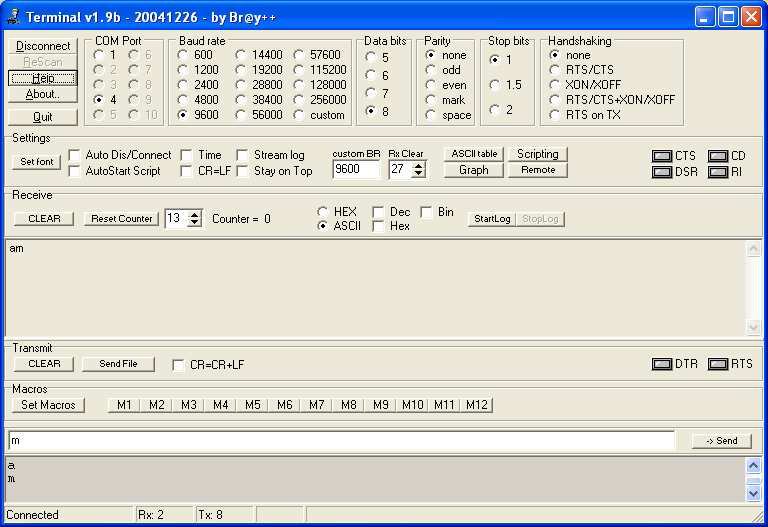
\includegraphics[width=300pt]{./Imagenes/Documentos/ArduinoNotebook_img14.png}
	\caption[Hyperterminal]{Software terminal para realizar comunicaciones}
\end{figure}

Seleccionar el puerto que estamos utilizando con la tarjeta, la velocidad de transferencia y el formato de salida de los datos. Y finalmente conectar...\\
Se puede realizar una comprobación con el siguiente programa mostrado a continuación.
\textbf{Nota}: El programa de monitorización de datos está ocupando el puerto utilizado para la conexión a la tarjeta, por lo que si quieres realizar una nueva descarga del programa, tendrás que desconectarte previamente de este último.\\
\begin{lstlisting}
/*by BARRAGAN <http://people.interaction-ivrea.it/h.barragan>
*Demuestra como leer un dato del puerto serie. Si el dato recibido es una 'H', la luz se
*enciende ON, si es una 'L', la luz se apaga OFF. Los datos provienen del PC o de un
*programa como Processing..
*created 13 May 2004 revised 28 Aug 2005
*/

char val; // variable que recibe el dato del puerto serie
int ledpin = 13; // LED conectado al pin 13

void setup()
{
   pinMode(ledpin, OUTPUT); // pin 13 (LED)actua como SALIDA
   Serial.begin(9600);    // inicia la comunicacion con el puerto serie a 9600bps
}

void loop()
{
   if( Serial.available() )    // si hay dato e el puerto lo lee
   {
      val = Serial.read();    // lee y almacena el dato en 'val'
   }
   if( val == 'H' )    //su el dato recibido es 'H'
   {
      digitalWrite(ledpin, HIGH); //activa el LED
   } else {
      digitalWrite(ledpin, LOW); // en caso contrario lo desactiva
   }
   delay(100);     // espera 100ms para una nueva lectura
}
\end{lstlisting}
Para probar este programa bastará con iniciar el programa que actúe de “terminal de comunicación” Hyperterminal de Windowws o el programa mostrado anteriormente y podemos enviar los datos y comprobar como actúa.

\section{Envío a petición (toma y dame)}

Cuando se envía más de un dato del Arduino a otro sistema es necesario implementar reglas de comunicación adicionales para poder distinguir a que dato corresponde cada uno de los paquetes de bytes recibidos. Una manera simple y eficiente de hacer esto es jugando al “toma y dame”. Arduino no enviará los valores de los sensores hasta que Processing no le envíe también un valor por el puerto serial y Processing, a su vez, no enviara ese valor hasta no tener los datos que espera completos.\\
Este sería el código para Arduino usando tres potenciómetros en los últimos tres pines analógicos del ATmega:
\begin{figure}[!htp]
	\centering
	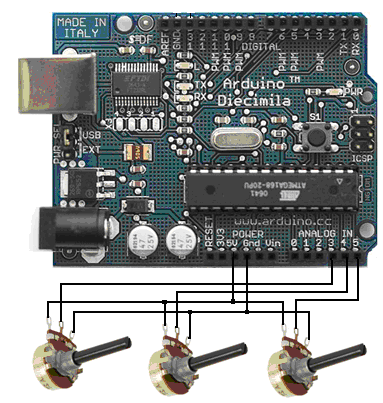
\includegraphics[width=100pt]{./Imagenes/Documentos/ArduinoNotebook_img15.png}
	\caption[Circuito Arduino con potenciometros]{Circuito de Arduino con potenciometros}
\end{figure}
Codigo para cargar en la tarjeta Arduino desde el IDE Arduino
\begin{lstlisting}
int pot1= 0;     // valores de los sensores analogicos
int pot2= 0;
int pot3= 0;
int inByte = 0;     // valor entrante de Processing

void setup()
{
   Serial.begin(9600);
}

void loop()
{
   if (Serial.available() > 0) { // solo si algo ha llegado

      inByte = Serial.read();    // lo lee

      // hace la lectura de los sensores en pines 3,4y5 (analogos)

      pot1 = analogRead(3)/4; pot2 = analogRead(4)/4; pot3 = analogRead(5)/4;

      // y los envia

      Serial.print(pot1, BYTE); Serial.print(pot2, BYTE); 
      Serial.print(pot3, BYTE);
   }
}
\end{lstlisting}
Una vez cargado este programa en la tarjeta Arduino está en disposición de enviar los datos de las lecturas de los potenciómetros cuando le sean demandados por el programa que los requiera. En nuestro ejemplo vamos a escribir un programa en el IDE Processing y será este el que se ocupe de leer los datos y con ellos modificar la posición de una bola que aparecerá en pantalla.\\
Será processing quién empezará el “toma y dame” y deberá reconocer cada dato. Este es el código:\\
\textbf{Código para Processing}\\
\begin{lstlisting}
import processing.serial.*;

Serial puerto;
int[] datosEntrantes = new int[3]; // arreglo para recibir los tres datos
int cuantosDatos = 0;     // contador
int posX, posY, posZ;     // posicion de un objeto 3D
boolean hayDatos = false;     // control de verdad

void setup() { size(400, 400, P3D); noStroke();


println(Serial.list());// puertos serie disponibles
puerto = new Serial(this, Serial.list()[0], 9600); // Configuracion del puerto
puerto.write(65);    // Envia el primer dato para iniciar el toma y dame
}


void draw() {
background(0); lights(); fill(30,255,20);
translate(width/2 + posX, height/2 + posY, posZ);
sphere(40);

if (hayDatos == false) { //si no hay datos envia uno
puerto.write(65);
}
}
// esta funcion corre cada vez que llega un dato serial


void serialEvent(Serial puerto) {
if (hayDatos == false) {

hayDatos = true;     // de ahora en adelante el dato de envio se dara por el toma y
dame
}
// Lee el dato y lo anade al arreglo en su ultima casilla
datosEntrantes[cuantosDatos] = puerto.read();
cuantosDatos++;
if (cuantosDatos > 2 ) { // Si ya hay tres datos en el arreglo

posX = datosEntrantes[0]; posY = datosEntrantes[1]; posZ = datosEntrantes[2];

println("Valores de los potenciometros: " + posX + "," + posY + "," + posZ);

puerto.write(65); // y envia para pedir mas

cuantosDatos = 0; // y todo empieza de nuevo
}

}
\end{lstlisting}


Aspecto del IDE Processing cuando está en funcionamiento el programa de captura de valores de los tres potenciómetros.